\documentclass[conference]{IEEEtran}
\usepackage{graphicx}

\begin{document}

\title{Revealing Unusual Events in GitHub Repositories}


\author{\IEEEauthorblockN{Xiyu Zhang}
\IEEEauthorblockA{a1673016\\School of Computer Science\\
The University of Adelaide\\
Adelaide, Australia\\
Email: \\a1673016@student.adelaide.edu.au}
\and
\IEEEauthorblockN{Jiexin Li}
\IEEEauthorblockA{a1714727\\School of Computer Science\\
The University of Adelaide\\
Adelaide, Australia\\
Email: \\a1714727@student.adelaide.edu.au}
\and
\IEEEauthorblockN{Tianshuo Zhang}
\IEEEauthorblockA{a1711997\\School of Computer Science\\
The University of Adelaide\\
Adelaide, Australia\\
Email: \\a1711997@student.adelaide.edu.au}
}


\maketitle


\begin{abstract}

At present, current large scale projects need developers to pay more attention on considering its details. In other words, developers need a useful tool to increase their awareness on what happened in their projects. Moreover, this project is based on previous researches by Christoph et al [1,2,3]. Its purpose is to implement a tool which can be able to detect unusual events in GitHub repositories. After that, showing results to developers in order to remind them what unusual events have existed in their repositories. During the whole process, we will cooperate with some mathematical students in order to try to define new types of unusual events. 
\end{abstract}



%%%%%%%%%%%%%%%%%%%%%%%%%%%%%%%%%%%%%%%%%%%%%%%%%%%%%%%%%%%%%%%%%%%%%%%%%%%%%%%%
\section{INTRODUCTION}

At present, a large amount of data is updated and uploaded every day in GitHub. As each project grows, developers need to think more and more about the details of the project. This makes it possible for developers to take into account some of the details of the project. And this can lead to a whole project's vulnerability even paralyze the project.\\

Christoph et al. [1] carried out data extraction and induction for 200 projects and 14 developers from GitHub on this issue. And through these data, the 6 operations were defined and named as unusual events and propose a reliable solution. For instance, adding multiple lines of code in a short period of time may lead to the emergence of bug. They believe that marking out unusual events can help developers better understand the progress of their own projects. In addition, it also helps them to take care of the easily overlooked details of the project. At the end of the paper by Christoph et al. [1], they suggest that they need to have a software to implement their ideas. We will implement this software and define more types of unusual events with them.

\section{Motivation}

In the process of modern software development. With the progress of the project, more and more details need to be paid more attention to them. This is not perfect for developers. This is likely to lead to obstacles to development. The purpose of this project is to reduce the occurrence of such a situation. Firstly, defining some unusual events that may be neglected. When these events happen, remind developers to improve the quality of projects. 

\subsection{Novelty Statement}

In the course of the project, we will do the statistics and analysis of the data with some mathematical students. Through experiments and studies to define new types of unusual events that are likely to be ignored.


\section{Background and Related work}

Nowadays, GitHub is the most famous code repository in the world, million, even billion, lines of code are stored in there. It is a Git repository based on web hosting service, and it can control all the distributed revision and manage source code. However, if you got a difficult issue which will take a long time to solve, many unusual comments will be attracted by some controversial pull requests, and adding and deleting files may happen because of disruptive commits.\\


Therefore, the commits, issues or pull requests cannot be possibly known immediately when the developer participates in a large software project. Nevertheless, there is no need to know all details which happen in the code. There are some high-level tools to attract developers’ attention for any activities in the code, for example Burn et al.’s Crystal [4] or WeCode [5] by Guimara ̃es and Silva. However, those tools provide limited information for the project.\\

Christoph et al.’s paper has defined some unusual events, for instance, an unusual commit message or uploading a lot of files [1]. They presented 140 users from 200 projects in GitHub. Finally, the very useful information is deleting, adding, modifying for the developers; meanwhile, the comments on issues and pull requests are also useful for them [1]. 



\section{Studied subjects / datasets}

The previous stage of our project may use the examples and data from the paper “Unusual Events in GitHub Repositories” written by Christoph et al.[1]. This paper has defined the unusual events to some extent. For the next step, we will collect data from other GitHub repositories as test sample, such as twbs/bootrap in GitHub. Firstly, we can detect consistently this repository as our original datasets because it big enough and many commits, pull requests, issues in it. In short, the first datasets we will get is from other repositories. At the later stage of this project, the datasets should be all the projects in GitHub.\\

At the same time, we will continuously define the unusual events for the next datasets. The next datasets will be the filtered datasets. This means that we will filter the original data from repositories by defined unusual events. Unfortunately, how to define an unusual event is difficult. The specific method to define unusual events should be discussed someone work or study in mathematics department. They will explain and build a formula for our project to define the unusual events, so that we can program the filter to wash the original datasets.


\section{Details of Expected Deliverables}
\subsection{The flow chart}
Our project process as Figure 1. Firstly, in order to detective unusual events, we need to get authorization from GitHub as a function of authorization login. After this step, we can get different GitHub APIs after authorization and using these APIs to access all repositories as the original data, and then collecting the original data and storing them into our database. Next, we will analyze all data, in order to get unusual events as the selected data. Finally, showing that on the web interface.

\begin{figure}[!ht]
\centering
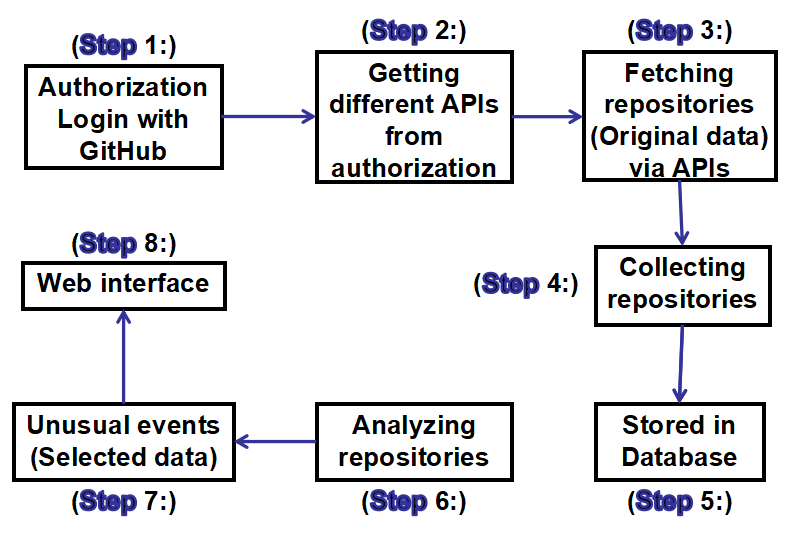
\includegraphics[scale=0.5]{methodology}
\caption{The project process}
\end{figure}

\subsection{Architecture}
For the architecture, our project will be hosted on AWS (Amazon Web Service) and our local database will be also deployed on RDS (Relational Database Service) which is a database service belong to AWS. However, in the beginning, we were implement different functions at local environment. As previous mentioned, the first function is to sign in with GitHub and all data such as user profile are stored in database. After that, we will code with these APIs to collect repositories and analyze them in order to get unusual events. Lastly, storing it into RDS and displaying that to users. Once we finished all functions, we will put thew whole project into AWS. Additionally, the architecture as Figure 2.

\begin{figure}[!ht]
\centering
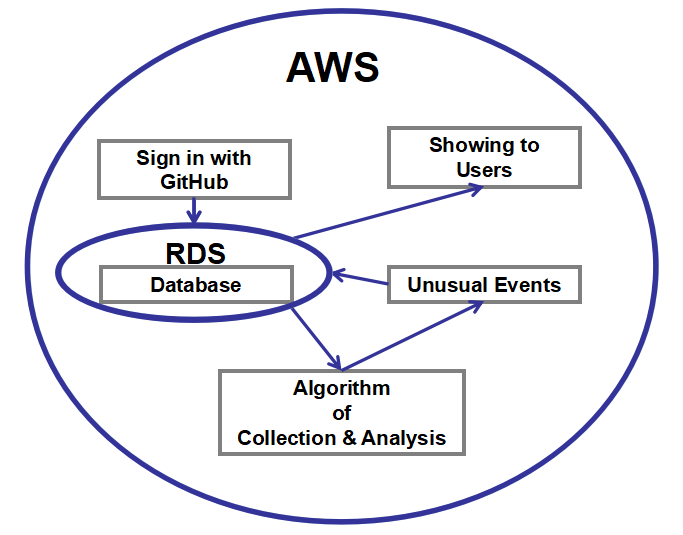
\includegraphics[scale=0.5]{architecture}
\caption{Architecture}
\end{figure}

\subsection{Milestones}
The ultimate goal of this project is to complete a system. Moreover, according to the flow chart and architecture, we have made 5 milestones on GitHub in order to help us to finish our deliverables on time.

\bigskip
\begin{itemize}
\item Find out the unusual events in the GitHub project;
\item Can be reviewed in the results list of different events;
\item Dynamic updates are displayed for the results of unusual events.
\end{itemize}
\bigskip
Temporarily, for the implementation of these functions, we have a few current deliverable plans:\\

\paragraph{\textbf{Milestone 1}}
\textbf{(AWS, the front-end demo and authorization)} We will deploy all functions for AWS and a front-end demo. After that, we will implement the authorization function, in order to get ready for collecting data from GitHub.\\

\paragraph{\textbf{Milestone 2}}
\textbf{(RDS and local database)} We will deploy RDS. After that, designing and implementing a local database, in order to store data from GitHub. Once we did it, we will get ready to collect data from GitHub. If possible, we can add an additional function of selecting projects with download button. \\

\paragraph{\textbf{Milestone 3}}
\textbf{(Collectors)} We will implement the function of collecting data. Once the data can be successfully collected, we will implement the function to analyze them. \\

\paragraph{\textbf{Milestone 4}}
\textbf{(Analyzers)} We will analyze all original data, and trying to get unusual events after analysis. If success, it can prove that our database is done, and then we can put the local database into RDS.\\

\paragraph{\textbf{Milestone 5}}
\textbf{(showing unusual events \& prototype)} We will test our prototype if it can be able to show unusual events on dashboard. After that, the whole prototype will be deployed on AWS.\\

\subsection{Specific details}
\subsubsection{The front-end demo}
After design, our front-end demo like Figure 3. Specifically, users profile will be shown on the left-top corner, status are displayed in the middle and the most important part of unusual events are put in the bottom. However, this is only a prototype for our front-end, we might change the layout for that.

\begin{figure}[!ht]
\centering
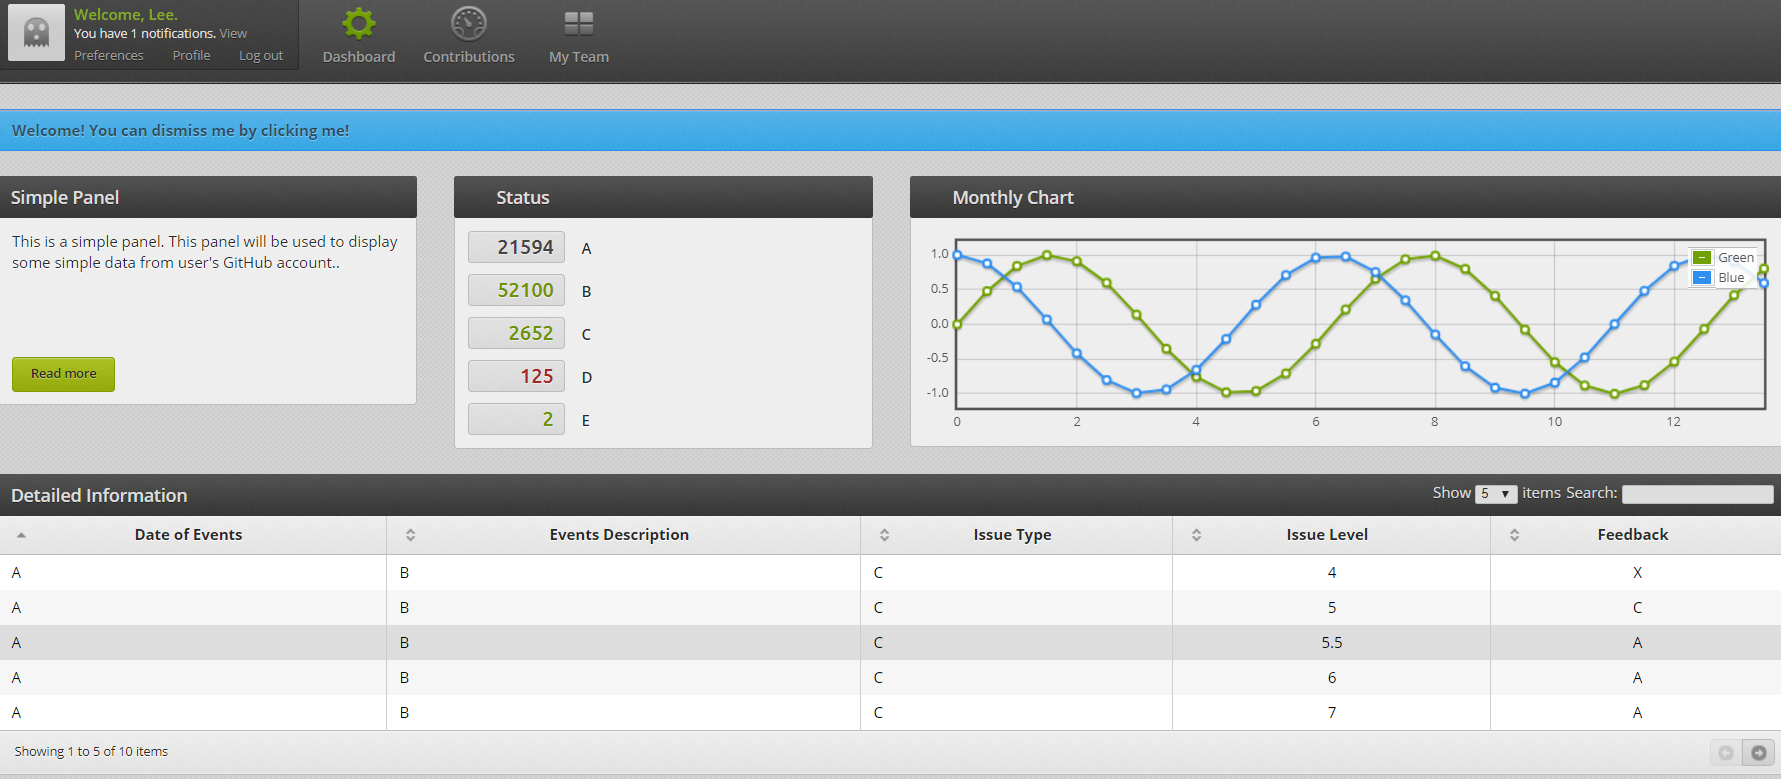
\includegraphics[scale=0.2]{the_front-end_demo}
\caption{The prototype of the front-end}
\end{figure}

\subsubsection{APIs}
In our project, one of the most important steps is to get authorization from users. Moreover, we have implemented this function and already got GitHub APIs after authorization. In addition, these APIs as Figure 4. Furthermore, we can store the data that what we want into our database by using APIs and then calling data when we need to analyze them. 

\begin{figure}[!ht]
\centering
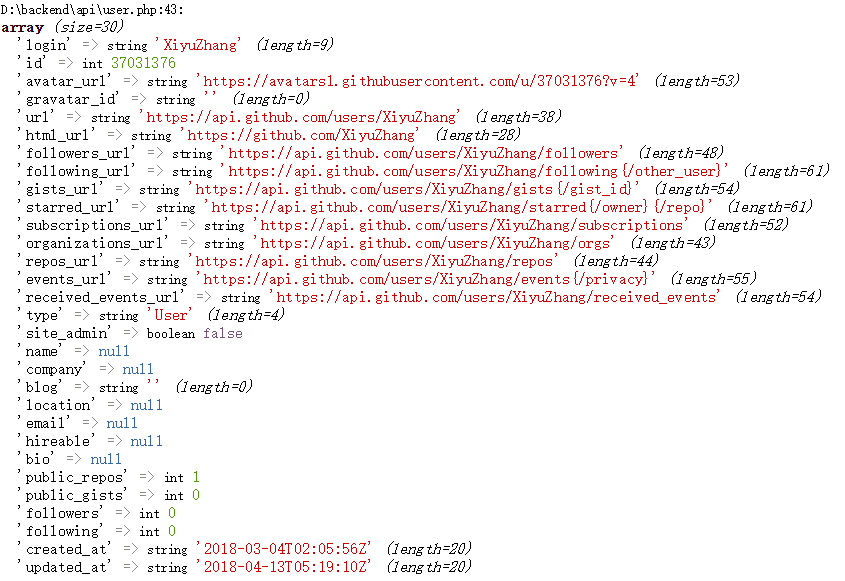
\includegraphics[scale=0.5]{APIs}
\caption{GitHub APIs (After authorization)}
\end{figure}

\subsubsection{Database}
This is an architecture for our database and we have 6 tables as Figure 5. In detail, account for user identification and it is unique. Moreover, the tables of commit, issue and pull\_request are for our original data. After analysis, the data will be store into the table of unusual\_events. Additionally, we have a table named feedback, this table for the function of comment on unusual events.

\begin{figure}[!ht]
\centering
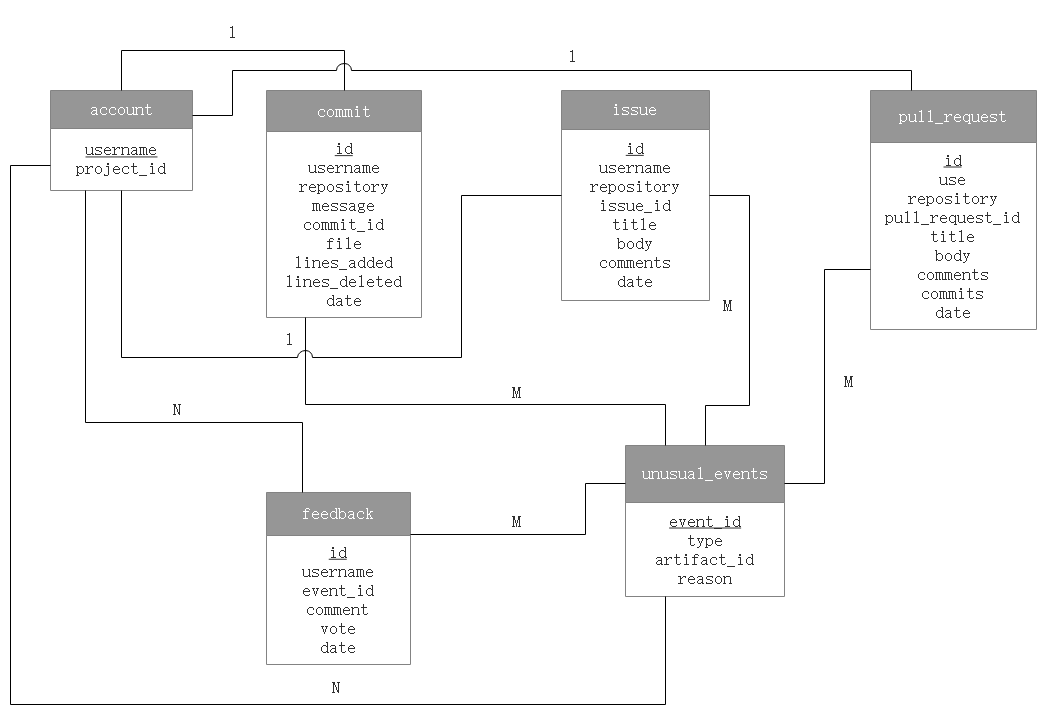
\includegraphics[scale=0.4]{database}
\caption{Architecture of our database}
\end{figure}

\subsubsection{The Back-end Process}
Above details are preparatory works. The real challenge is to implement each function and gathering all of them together. For this reason, wee have design a process for our back-end as Figure 6, in order to help us to implement the prototype of this project. In detail, this image is to describe that our project process in a simple way.\\

Firstly, We will use three layers framework combining with Model View Controller(MVC),which helps us to build a web application easier. The download in the dashboard.jsp page means to get the data we want from the GitHub project. In the web layer, DownloadDataServlet will be responded when the download button is pressed. The DownloadDataServlet will use the function in DataService to filter the data we want to save in the database. Finally, the selected data will be put into database by the function 'saveAllData' in the DataDao layer.\\

The second step is that there is a new page which has a view data button. When user press this button, UserDataListServlet will be responded to use the function 'findAllData()' in the UserDataService layer. Also, the dao layer is to do database operation; therefore, we use another function 'findAllData()' in DAO to get the user data. After that, data will be packaged as List type and transmit to the service layer. This is because the service layer is to deal with complicated transactions, so we will use 'unusual events algorithm' to select data that user wants. At the end of this step, data will be transmitted to the web layer and displayed on the page.

\begin{figure}[!ht]
\centering
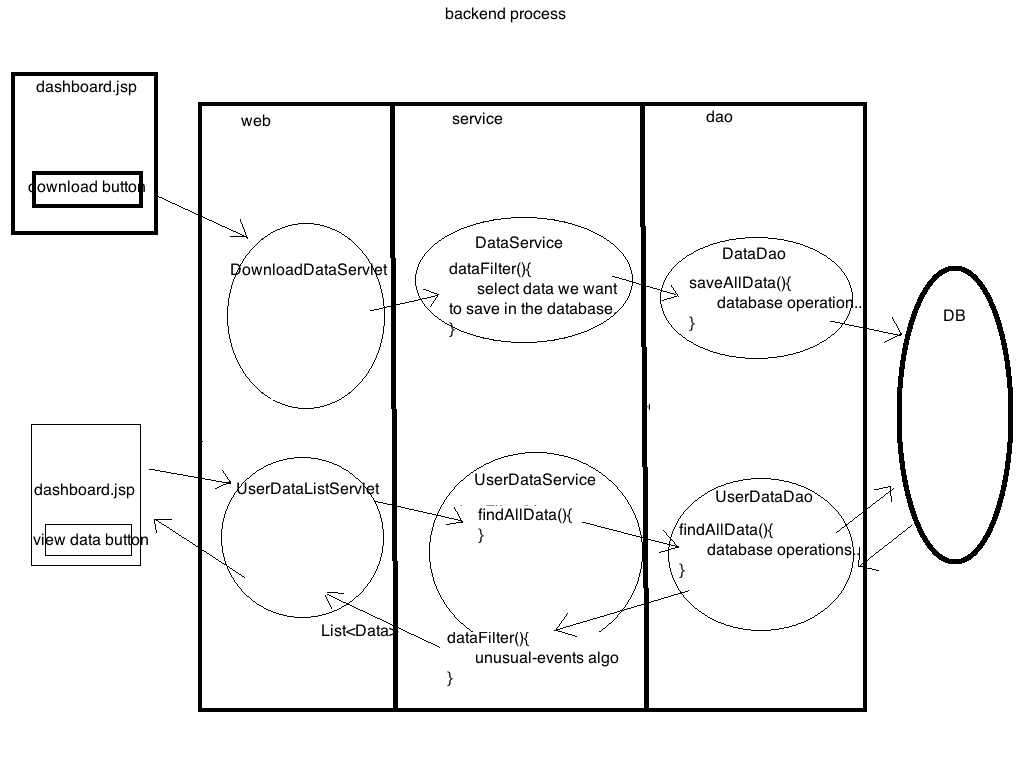
\includegraphics[scale=0.25]{back-end_process}
\caption{The process for back-end}
\end{figure}


\section{The Gantt Chart}
Since the first lecture of Software Engineering Project Part A at week 1, we have never stop to work on that. After the first lecture, all teammates decided the topic that “Revealing unusual events in GitHub repositories”. After that, we have read some related publications which is from our supervisor. Moreover, we analyzed some requirements for this project and confirmed that with our supervisor. And than, we started to design the front and back ends, also doing some practices with useful recommended tools such as AWS, in order to be more efficient in this project. In the process of development, we decided to implement the most basic functions. After discussion with supervisor, we are going to spend a few time to build the running environment of recommended tools in the beginning of development. Further, implementing the following functions step by step, such as the front-end interface, login with GitHub account, collecting needed data from GitHub and analyzing them and displaying unusual events on our dashboard. Lastly, we will use couple days to do testing before the due date of each milestone. The Gantt chart of the above process as Figure 7. In addition, the Gantt chart provides a comprehensive details for our project and listing consumed time for each step. We have finish all preparatory works of this project currently, and the remaining work is to implement this tool.


\begin{figure}[!ht]
\centering
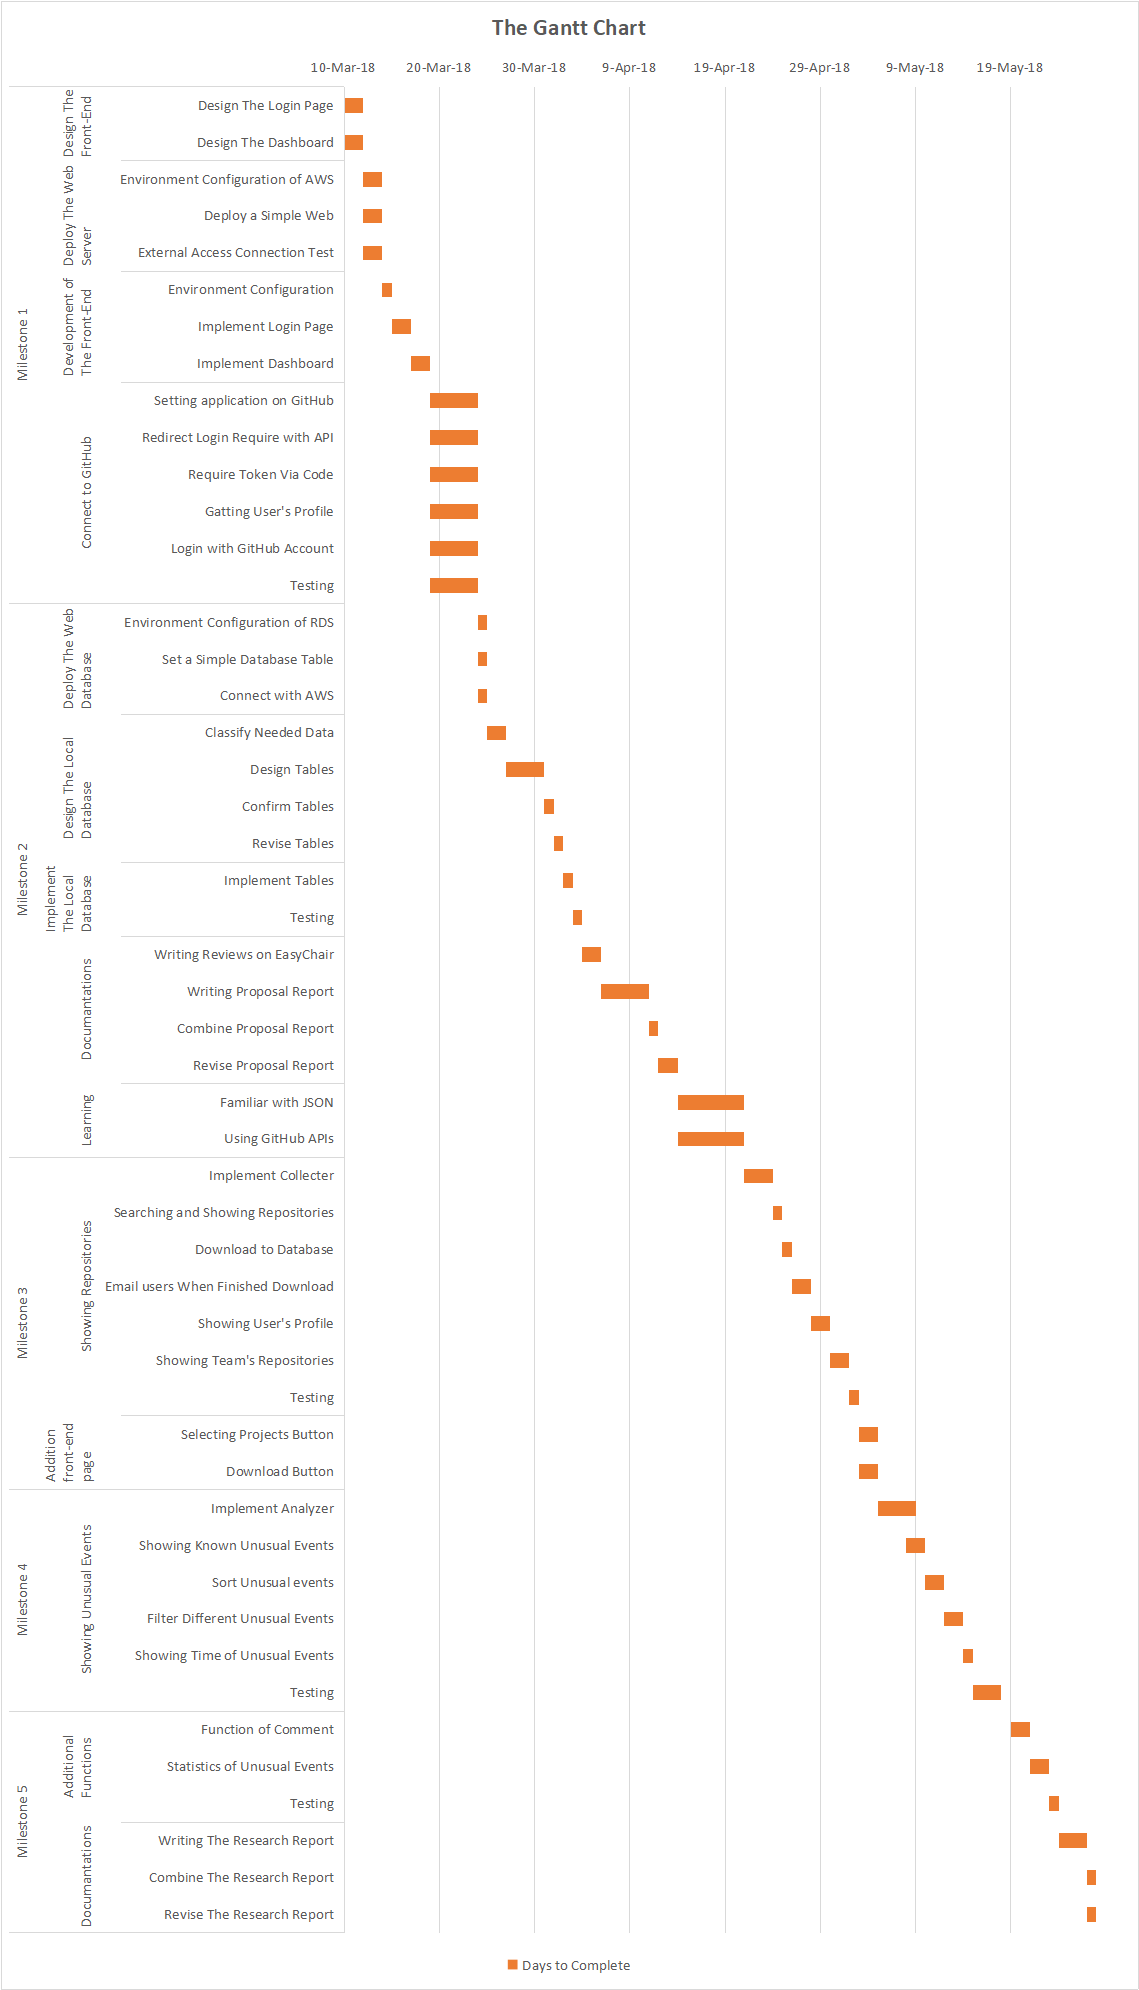
\includegraphics[scale=0.35]{the_Gantt_chart}
\caption{The Gantt chart for this project}
\end{figure}


\section{Individual Contributions}


\paragraph{\textbf{Xiyu Zhang (Responsibility: The back-end)}}
\medskip
\begin{itemize}
\item Design and Implement the back-end
\item Implement the authorization login with GitHub
\item Implement the Database
\item Combining documents
\end{itemize}
\bigskip

\paragraph{\textbf{Jiein Li (Responsibility: The front-end)}}
\medskip
\begin{itemize}
\item Design and Implement the front-end
\item Design the Database tables
\item Produce quality management
\end{itemize}
\bigskip

\paragraph{\textbf{Tianshuo Zhang (Responsibility: The back-end)}}
\medskip
\begin{itemize}
\item Connecting the GitHub API with the front-end
\item Algorithm of analyzing original data
\item Testing to the prototype
\end{itemize}


\begin{thebibliography}{99}

\bibitem{c1} Treude C, Leite L, Aniche M. Unusual Events in GitHub Repositories[J]. arXiv preprint arXiv:1710.01943, 2017.\\

\bibitem{c2} Treude C, Figueira Filho F, Kulesza U. Summarizing and measuring development activity[C]//Proceedings of the 2015 10th Joint Meeting on Foundations of Software Engineering. ACM, 2015: 625-636.\\

\bibitem{c3} Leite L, Treude C, Figueira Filho F. UEDashboard: awareness of unusual events in commit histories[C]//Proceedings of the 2015 10th Joint Meeting on Foundations of Software Engineering. ACM, 2015: 978-981.\\

\bibitem{c4} Y. Brun, R. Holmes, M. D. Ernst, D. Notkin, Proactive detection of collaboration conflicts, in: Proceedings of the 19th SIGSOFT Sympo- sium and the 13th European Conference on Foundations of Software Engineering, 2011, pp. 168–178. 
\bibitem{c5} M. L. Guimar ̃aes, A. R. Silva, Improving early detection of software merge conflicts, in: Proceedings of the 34th International Conference on Software Engineering, 2012, pp. 342–352. 


\end{thebibliography}


\end{document}